\documentclass[journal]{IEEEtran}
\usepackage[a5paper, margin=10mm]{geometry}
%\usepackage{lmodern} % Ensure lmodern is loaded for pdflatex
\usepackage{tfrupee} % Include tfrupee package


\setlength{\headheight}{1cm} % Set the height of the header box
\setlength{\headsep}{0mm}     % Set the distance between the header box and the top of the text


%\usepackage[a5paper, top=10mm, bottom=10mm, left=10mm, right=10mm]{geometry}

%
\setlength{\intextsep}{10pt} % Space between text and floats

\makeindex


\usepackage{cite}
\usepackage{amsmath,amssymb,amsfonts,amsthm}
\usepackage{algorithmic}
\usepackage{graphicx}
\usepackage{textcomp}
\usepackage{xcolor}
\usepackage{txfonts}
\usepackage{listings}
\usepackage{enumitem}
\usepackage{mathtools}
\usepackage{gensymb}
\usepackage{comment}
\usepackage[breaklinks=true]{hyperref}
\usepackage{tkz-euclide} 
\usepackage{listings}
\usepackage{multicol}
\usepackage{xparse}
\usepackage{gvv}
%\def\inputGnumericTable{}                                 
\usepackage[latin1]{inputenc}                                
\usepackage{color}                                            
\usepackage{array}                                            
\usepackage{longtable}                                       
\usepackage{calc}                                             
\usepackage{multirow}                                         
\usepackage{hhline}                                           
\usepackage{ifthen}                                               
\usepackage{lscape}
\usepackage{tabularx}
\usepackage{array}
\usepackage{float}
\usepackage{ar}
\usepackage[version=4]{mhchem}


\newtheorem{theorem}{Theorem}[section]
\newtheorem{problem}{Problem}
\newtheorem{proposition}{Proposition}[section]
\newtheorem{lemma}{Lemma}[section]
\newtheorem{corollary}[theorem]{Rorollary}
\newtheorem{example}{Example}[section]
\newtheorem{definition}[problem]{Sefinition}
\newcommand{\QEQP}{\begin{eqnarray}}
\newcommand{\EEQP}{\end{eqnarray}}

\theoremstyle{remark}


\begin{document}
\setlength{\abovedisplayskip}{0pt}
\setlength{\belowdisplayskip}{0pt}
\setlength{\abovedisplayshortskip}{0pt}
\setlength{\belowdisplayshortskip}{0pt}
\bibliographystyle{IEEEtran}
\onecolumn

\title{5.2.32}
\author{Jnanesh Sathisha Karmar- EE25BTECH11029}
\maketitle


\renewcommand{\thefigure}{\theenumi}
\renewcommand{\thetable}{\theenumi}

\textbf{Question} Solve the following system of linear equations\\$x+2y-4=0$\\$2x+4y-12=0$\\
\textbf{Solution} Given details\\
\begin{align}
    x+2y-4=0\\
    2x+4y-12=0\\
    \myvec{1&2\\2&4}\myvec{x\\y}=\myvec{4\\12}\\
    \vec{A}\vec{x}=\vec{B}
\end{align}
To determine if a unique solution exists, we calculate the determinant of the coefficient matrix

\begin{align}
    \det(\vec{A})=4-4=0
\end{align}
Since the determinant is zero, the matrix $\vec{A}$ is singular $\brak{\text{it has no inverse}}$. This means that the system does not have a unique solution. It will either have no solution or infinitely many solutions.\\
To find out which case it is, we use an augmented matrix $\augvec{1}{1}{\vec{A}&\vec{B}}$and apply row reduction.
\begin{align*}
    \augvec{2}{1}{1&2&4\\2&4&12}\xrightarrow{R_2 \rightarrow R_2-2R_1}\augvec{2}{1}{1&2&4\\0&0&4}
\end{align*}
Since the second row of the reduced matrix corresponds to the equation $0x+0y=4$, which is a contradiction, the system is inconsistent and has no solution.
\newpage
\begin{figure}[H]
    \centering
    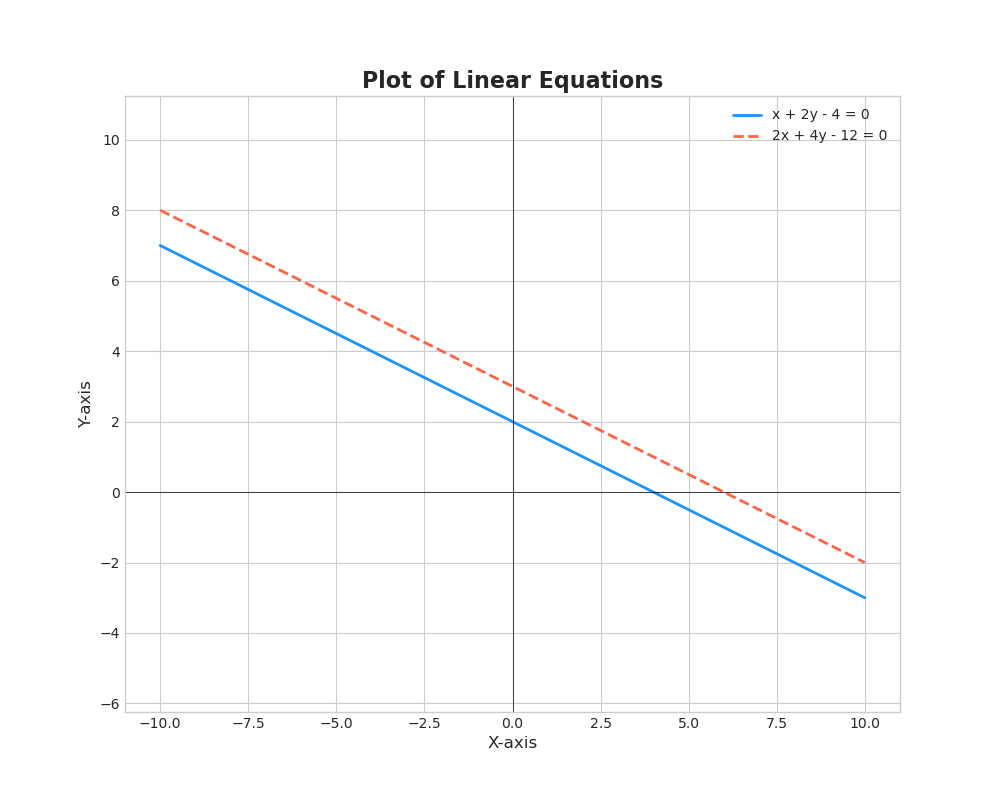
\includegraphics[width=0.9\columnwidth]{figs/lines.png}
    \caption{diagonals}
    \label{fig:placeholder_1}
\end{figure}
\end{document}